% Provenance (never printed): see sources/outline_sources.md (Year 3: gravity, magnetic,
% seismic, resistivity and ground-penetrating-radar surveys; data processing and
% uncertainty; a mapping project).
% Brief: sources/book5/BRIEFS.md, ch. 31. Curves from figdata/bachelor-3/gravity_granite.py
% (prism model of the Varden granite of figdata/shared/region.py), magnetic_dyke.py (2-D
% dyke; the Varden dolerite dyke of the Sync 3 ruling, buried below the unconformity),
% resistivity_sounding.py (Pekeris transform and image series) and gpr_radargram.py.
% Physical-property ranges and survey practice from the GPG open textbook (CC BY 4.0) and
% Keys (1990). Exercise and problem values in the Book 5 scratch calculator calc/ch31.py.
\chapter{क्षेत्र और प्रयोगशाला विधियाँ III}\label{ch:b3:field-lab-methods-3}

एक भूभौतिकी दल वार्डन पहाड़ियों की घाटी में एक सप्ताह बिताता है, यह एक काल्पनिक क्षेत्र है
जिसका भूवैज्ञानिक मानचित्र पुस्तक 3 (स्नातक वर्ष 1) ने अपने
भूवैज्ञानिक मानचित्रों वाले अध्याय में बनाया था। मानचित्र में एक ग्रेनाइट का अनावरण दिखता है
घाटी के किनारों पर, शिस्ट के बीच, उस बलुआ पत्थर के नीचे जो
दोनों ओर टिका है। ग्रेनाइट कवर के नीचे कहाँ जाता है, कितनी दूर
तक फैला है और कितनी गहराई तक पहुँचता है, यह किसी ने नहीं देखा।
दल के पास एक गुरुत्वमापी, दो चुंबकत्वमापी, इलेक्ट्रोड की एक केबल और एक रडार
छोटी गाड़ी पर रखा है। इनमें से कोई भी उपकरण चट्टान को नहीं देखता: प्रत्येक
सतह पर एक क्षेत्र मापता है---गुरुत्व, चुंबकीय क्षेत्र, एक विद्युत विभव,
किसी रेडियो स्पंद की प्रतिध्वनि---जिसे नीचे की चट्टानें विक्षुब्ध करती हैं।
सप्ताह के अंत तक दल वह ग्रेनाइट खींच सकता है जिसे उसने कभी नहीं देखा,
बता सकता है कि घाटी के तल पर जलोढ़ कितना गहरा है, और एक ऐसे चुंबकीय पिंड की
रिपोर्ट दे सकता है जो किसी मानचित्र में नहीं था।

यह अध्याय उसी सप्ताह का अनुसरण करता है। यह हर विधि को बारी-बारी से लेता है, एक माप के रूप में
उसके संशोधनों सहित, और कुछ ऐसे पिंडों के साथ एक \omterm{def:b3:seismology-imaging:inverse}{अग्र समस्या} के रूप में जिनके क्षेत्र
ठीक-ठीक परिकलित किए जा सकते हैं; फिर यह बताता है कि किसी सर्वेक्षण की त्रुटियाँ कैसे
जुड़ती हैं और आँकड़ों का एक ही प्रकार किसी मॉडल को कम ही
निश्चित करता है; और यह वार्डन सर्वेक्षण पर समाप्त होता है, जहाँ सभी विधियाँ
एक साथ रखी जाती हैं।

\begin{recall}
गुरुत्व विसंगति, मुक्त-वायु और बूगेर सुधार और विसंगतियाँ
तथा सामान्य गुरुत्व पुस्तक 3 (स्नातक वर्ष 1) में, उसके समस्थिति और गुरुत्व वाले अध्याय में हैं;
\omterm{def:b3:field-lab-methods-3:gravimeter}{सापेक्ष गुरुत्वमापी} का सर्वेक्षण लूप
\cref{ch:b3:gravity-geodesy} में वर्णित है। मुख्य क्षेत्र, उसका नति कोण,
\omterm{thm:b3:palaeomagnetism:dipole}{द्विध्रुव सूत्र} और \omterm{def:b3:palaeomagnetism:igrf}{अंतरराष्ट्रीय भू-चुंबकीय संदर्भ क्षेत्र}
\cref{ch:b3:palaeomagnetism} में हैं। प्रतिरोधकता, ओम का
नियम, आपेक्षिक विद्युतशीलता, विद्युत-चुंबकीय तरंगें, चुंबकन और चुंबकीय
प्रवृत्ति भौतिकी की पुस्तकों में हैं, और गुरुत्व के लिए गॉस का प्रमेय
उनके साथ। \omterm{def:b3:exploration-seismology:surveys}{भूकंपीय अपवर्तन सर्वेक्षण}
\cref{ch:b3:exploration-seismology} में हैं; अग्र और प्रतिलोम समस्याएँ तथा भारित न्यूनतम वर्ग
\cref{ch:b3:seismology-imaging} में; छिद्रता विद्यालय की पुस्तकों में और
\omterm{def:b3:facies-models:wireline}{वायरलाइन लॉग} \cref{ch:b3:facies-models} में।
अनिश्चितताओं का प्रसार रसायन और गणित की पुस्तकों में है।
\end{recall}

\section{गुरुत्व सर्वेक्षण}\label{sec:b3:field-lab-methods-3:gravity}

वे विसंगतियाँ जिन्हें एक गुरुत्व सर्वेक्षण खोजता है, छोटी होती हैं। भूमध्य रेखा पर गुरुत्व
लगभग \qty{978000}{\milli\gal} है; बड़ी संरचनाएँ उसे
सैकड़ों मिलीगल से, एक लवण गुंबद लगभग दस से, एक अयस्क पिंड लगभग
एक से, और भू-तकनीकी सर्वेक्षण के लक्ष्य कुछ
सौवें भाग से। भूभौतिकीविद् मिलीगल में मापते हैं,
या \qty{0.1}{\milli\gal} की गुरुत्व इकाइयों में; एक उपयोगी सर्वेक्षण
को $g$ के सौ करोड़ में एक भाग के अंतर को विभेदित करना होगा।
% ledger: gpg:grav-units, gpg:grav-sizes

\begin{definition}[सापेक्ष गुरुत्वमापी; उपकरणीय विचलन]\label{def:b3:field-lab-methods-3:gravimeter}
एक \emph{सापेक्ष गुरुत्वमापी}\index{सापेक्ष गुरुत्वमापी} एक ऐसा उपकरण है
जो स्टेशनों के बीच गुरुत्व के अंतर मापता है: एक स्प्रिंग पर लगा द्रव्यमान,
जिसे एक दूसरे, समायोज्य बल द्वारा शून्य स्थिति पर रखा जाता है; उस बल का
डायल पाठ्यांक, एक अंशांकन स्थिरांक से गुणा करने पर, गुरुत्व देता है
मिलीगल में, एक अज्ञात स्थिरांक तक। इसका \emph{उपकरणीय
विचलन}\index{उपकरणीय विचलन} एक स्थिर स्टेशन पर उसके पाठ्यांक का धीमा परिवर्तन है,
जो स्प्रिंग के विसर्पण, तापमान और झटकों से होता है; इसे कुछ घंटों बाद
फिर से पढ़कर मापा जाता है, एक ऐसे स्टेशन को जो पहले पढ़ा जा चुका है,
वह \emph{आधार स्टेशन}।
\end{definition}
% ledger: gpg:gravimeter, gpg:grav-survey

एक क्षेत्रीय गुरुत्वमापी कई दसियों हज़ार
मिलीगल की परास को ढकता है और अपने सर्वोत्तम रूप में लगभग \qty{0.01}{\milli\gal} तक पढ़ता है;
परिवहन के बाद परास को फिर से शून्य पर सेट करना होता है। इस सटीकता पर हर स्टेशन की ऊँचाई
उसके पाठ्यांक जितनी ही मायने रखती है: \qty{3.3}{cm} की ऊँचाई त्रुटि
\qty{0.01}{\milli\gal} को बिगाड़ देती है, इसलिए स्थितियाँ
उपग्रह ग्राहियों या सेंटीमीटर तक सही स्तर से मापी जाती हैं। आधार स्टेशन को
हर कुछ घंटों पर फिर से लिया जाता है। ठोस-पृथ्वी ज्वार, जो
\qty{0.3}{\milli\gal} तक पहुँच सकता है, उन घंटों में इतनी धीमी गति से बदलता है
कि उसे विचलन के साथ हटाया जा सकता है।
% ledger: gpg:gravimeter, gpg:grav-survey, gpg:grav-sizes

\begin{method}[गुरुत्व लूप का समानयन]\label{met:b3:field-lab-methods-3:loop}
एक लूप एक आधार स्टेशन से शुरू होता है और उसी पर समाप्त होता है, जिसे समय $t_0$ और $t_1$ पर पढ़ा जाता है।
\begin{enumerate}
  \item दो आधार पाठ्यांकों से विचलन दर $(r_1 - r_0)/(t_1 - t_0)$ परिकलित कीजिए;
        इसमें ज्वार शामिल है।
  \item हर पाठ्यांक से $t_0$ के बाद संचित विचलन घटाइए,
        $r - (t - t_0)(r_1 - r_0)/(t_1 - t_0)$, और आधार पाठ्यांक घटाइए:
        यह आधार के सापेक्ष गुरुत्व है।
  \item आधार से स्टेशन की ऊँचाई $\Delta h$ का संशोधन कीजिए:
        मुक्त-वायु सुधार $\qty{0.3086}{\milli\gal.m^{-1}}
        \times\Delta h$ जोड़िए और बूगेर सुधार
        $\qty{0.1119}{\milli\gal.m^{-1}}\times\Delta h$ (घनत्व
        \qty{2670}{kg.m^{-3}}) घटाइए, अर्थात $0.1967\,\Delta h$ जोड़िए।
  \item आधार से $\Delta y$ दूरी पर उत्तर में स्थित स्टेशन के लिए सामान्य गुरुत्व का
        परिवर्तन घटाइए, $\qty{0.811}{\milli\gal.km^{-1}}
        \times\sin 2\varphi\times\Delta y$।
  \item हर स्टेशन का \omterm{def:b3:field-lab-methods-3:terrain}{भू-भाग संशोधन} जोड़िए।
\end{enumerate}
परिणाम आधार के सापेक्ष बूगेर विसंगति है। आधार को
ज्ञात निरपेक्ष गुरुत्व वाले किसी स्टेशन से जोड़ने पर स्वयं विसंगति प्राप्त होती है।
\end{method}
% ledger: gpg:grav-survey, gpg:terrain

बूगेर सुधार स्टेशन और संदर्भ तल के बीच के भूभाग को
एक समतल स्लैब मानता है। वास्तविक उच्चावच में यह दो तरह से गलत है:
स्टेशन के ऊपर उठती एक पहाड़ी ऊपर की ओर खींचती है और
पाठ्यांक को घटाती है, और स्टेशन के नीचे गिरती एक घाटी
स्लैब में ऐसी चट्टान गिनी जाती है जो वहाँ है ही नहीं।

\begin{definition}[भू-भाग संशोधन]\label{def:b3:field-lab-methods-3:terrain}
किसी गुरुत्व स्टेशन का \emph{भू-भाग संशोधन}\index{भू-भाग संशोधन} वह आकर्षण है जो
स्टेशन पर बूगेर स्लैब से उच्चावच के विचलन लगाते हैं:
स्टेशन के स्तर से ऊपर की पहाड़ियाँ, और उसके नीचे की घाटियाँ,
जिन्हें स्लैब के घनत्व से गिना जाता है। दोनों ही स्लैब की तुलना में
मापे गए गुरुत्व को घटाते हैं, इसलिए संशोधन
सदैव जोड़ा जाता है।
\end{definition}

पहले इसे हैमर चार्ट और सारणियों की सहायता से हाथ से,
स्टेशन से बाहर की ओर क्षेत्र-दर-क्षेत्र परिकलित किया जाता था; आज यह अंकीय उन्नयन
मॉडल से परिकलित होता है। तीव्र उच्चावच से दूर यह कम ही \qty{1}{\milli\gal} से अधिक होता है,
परंतु स्टेशन के निकट के क्षेत्रों को सही निकालना कठिन होता है, और
संशोधन शायद ही \qty{0.2}{\milli\gal} से बेहतर परिशुद्धता से ज्ञात होता है।
% ledger: gpg:terrain, gpg:grav-sizes

\subsection{सरल पिंडों की विसंगतियाँ}

गुरुत्व की \omterm{def:b3:seismology-imaging:inverse}{अग्र समस्या} एक योग है: किसी पिंड का प्रत्येक अवयव, जिसका
घनत्व अंतर $\Delta\rho$ है, न्यूटन के नियम से स्टेशन को आकर्षित करता है, और
सर्वेक्षण योग के ऊर्ध्वाधर घटक को मापता है। कुछ पिंड इसे
बंद रूप में देते हैं।

\begin{theorem}[गोला और क्षैतिज बेलन]\label{thm:b3:field-lab-methods-3:sphere}
अपने केंद्र के ठीक ऊपर के बिंदु से क्षैतिज दूरी $x$ पर, एक दबा हुआ गोला
जिसका अधिक द्रव्यमान $\Delta m$ है और जिसका केंद्र गहराई $z$ पर है, वह
विसंगति देता है:
\[
\Delta g(x) = \frac{G\,\Delta m\,z}{(x^2 + z^2)^{3/2}} ,
\]
और विसंगति अपने शिखर के आधे पर $x_{1/2} = z\sqrt{2^{2/3} - 1}$ पर गिरती है,
इसलिए $z = 1.305\,x_{1/2}$ होता है। एक लंबा क्षैतिज बेलन, जिसका अधिक द्रव्यमान
प्रति इकाई लंबाई $\lambda$ है, और जिसका अक्ष गहराई $z$ पर है, वह
स्ट्राइक के आर-पार यह देता है:
\[
\Delta g(x) = \frac{2G\lambda z}{x^2 + z^2} ,
\]
और $z = x_{1/2}$ होता है।
\end{theorem}

\begin{proof}
ऐसे गोले के बाहर, जिसका घनत्व केवल केंद्र से दूरी पर निर्भर करता है,
आकर्षण उतना ही होता है जितना केंद्र पर रखे उसके द्रव्यमान का (कोश प्रमेय,
जो गॉस प्रमेय का एक परिणाम है)। स्टेशन पर इसका परिमाण
$G\Delta m/(x^2 + z^2)$ है, और ऊर्ध्वाधर घटक में गुणक
$z/\sqrt{x^2 + z^2}$ आता है। $\Delta g(x_{1/2}) =
\Delta g(0)/2$ रखने पर $(1 + x_{1/2}^2/z^2)^{3/2} = 2$ प्राप्त होता है, और इसी से नियम निकलता है। बेलन के लिए,
त्रिज्या $r$ के सह-अक्षीय बेलन पर गॉस का प्रमेय
$2G\lambda/r$ का क्षेत्र, और ऊर्ध्वाधर घटक $2G\lambda z/r^2$ देता है;
शिखर का आधा तब प्राप्त होता है जब $x^2 + z^2 = 2z^2$।
\end{proof}
% ledger: gpg:half-width

जो पिंड गोला नहीं है, उसकी भी एक अर्ध-चौड़ाई होती है, और तब नियम
पिंड की नहीं, बल्कि एक तुल्य गोले की गहराई देता है। यह नियम
एक प्रथम अनुमान है, जो किसी भी मॉडल के फिट होने से पहले बनाया जाता है।

\begin{proposition}[अपने अक्ष पर ऊर्ध्वाधर बेलन]\label{prop:b3:field-lab-methods-3:vcyl}
त्रिज्या $a$ और घनत्व अंतर $\Delta\rho$ वाला एक ऊर्ध्वाधर बेलन, जिसका
ऊपरी और निचला सिरा स्टेशन के नीचे गहराई $z_1 < z_2$ पर है,
अपने अक्ष पर यह देता है:
\[
\Delta g = 2\pi G\Delta\rho\left[(z_2 - z_1) + \sqrt{z_1^2 + a^2}
           - \sqrt{z_2^2 + a^2}\right] .
\]
$a \to \infty$ पर यह बूगेर स्लैब $2\pi G\Delta\rho(z_2 - z_1)$ है;
सतह से बहुत अधिक गहराई तक के बेलन के लिए यह
$2\pi G\Delta\rho\,a$ की ओर प्रवृत्त होता है।
\end{proposition}

\begin{proof}
त्रिज्या $a$ और मोटाई $\mathrm{d}z$ की एक चकती, जो गहराई $z$ पर है, अपने अक्ष पर स्थित
एक बिंदु को $2\pi G\Delta\rho\,\mathrm{d}z\,(1 -
z/\sqrt{z^2 + a^2})$ के बल से आकर्षित करती है, जो वलय का आकर्षण है, जिसे
त्रिज्या पर समाकलित किया जाता है। $z_1$ से $z_2$ तक समाकलन करने पर कोष्ठक प्राप्त होता है। जब $a \to
\infty$ होने पर, स्थिर गहराइयों पर, $\sqrt{z_1^2 + a^2} - \sqrt{z_2^2 + a^2} =
(z_1^2 - z_2^2)/(\sqrt{z_1^2 + a^2} + \sqrt{z_2^2 + a^2}) \to 0$; जब
$z_1 = 0$ और $z_2 \to \infty$, $z_2 - \sqrt{z_2^2 + a^2} \to 0$ और
कोष्ठक $a$ की ओर प्रवृत्त होता है।
\end{proof}

\begin{proposition}[गुरुत्व मानचित्र से अधिक द्रव्यमान]\label{prop:b3:field-lab-methods-3:gauss}
क्षैतिज तल के पूर्णतः नीचे स्थित पिंड का आकार चाहे कुछ भी हो,
उसका अधिक द्रव्यमान इस प्रकार है:
\[
\Delta m = \frac{1}{2\pi G}\iint \Delta g\,\mathrm{d}A ,
\]
समाकल पूरे तल को आच्छादित करता है।
\end{proposition}

\begin{proof}
बिंदु द्रव्यमान $m$ के लिए, जो गहराई $z$ पर है, जहाँ $r$ क्षैतिज दूरी है,
$\iint \Delta g\,\mathrm{d}A = \int_0^\infty
Gmz\,(r^2 + z^2)^{-3/2}\,2\pi r\,\mathrm{d}r = 2\pi Gm$: गॉस प्रमेय के फ़्लक्स का आधा
$4\pi Gm$ तल को पार करता है। एक पिंड बिंदु-द्रव्यमानों का योग होता है,
और समाकल रैखिक होता है।
\end{proof}

प्रमेय द्रव्यमान देता है, आकार कभी नहीं; और मानचित्र तल के केवल एक भाग को
आच्छादित करता है, जबकि गहरे पिंड की विसंगति धीरे-धीरे क्षीण होती है, इसलिए
मानचित्र से प्राप्त द्रव्यमान बहुत छोटा निकलता है, जब तक उसके किनारे
किसी मॉडल से विस्तारित न किए जाएँ।

\begin{omfigure}
\begin{tikzpicture}
\begin{axis}[axis equal image, xmin=1.5, xmax=5.5, ymin=2.6, ymax=5.7, width=0.86\linewidth,
  tick label style={font=\scriptsize}, xlabel={पूर्व (km)}, ylabel={उत्तर (km)},
  label style={font=\small}, unbounded coords=jump]
% geology of the region (figdata/shared/region.py), faded
\addplot[lith schist, draw=black!50, line width=0.2pt, even odd rule, opacity=0.45] table {figdata/out/shared-region-unit-schist.dat};
\addplot[lith granite, draw=black!50, line width=0.2pt, even odd rule, opacity=0.45] table {figdata/out/shared-region-unit-granite.dat};
\addplot[om lith={icsTriassic!35}{om sand}, draw=black!50, line width=0.2pt, even odd rule, opacity=0.45] table {figdata/out/shared-region-unit-sandstone.dat};
\addplot[om lith={icsJurassic!40}{om limestone}, draw=black!50, line width=0.2pt, even odd rule, opacity=0.45] table {figdata/out/shared-region-unit-limestone.dat};
\addplot[om lith={icsJurassic!15}{om shale}, draw=black!50, line width=0.2pt, even odd rule, opacity=0.45] table {figdata/out/shared-region-unit-shale.dat};
\addplot[lith alluvium, draw=black!50, line width=0.2pt, even odd rule, opacity=0.45] table {figdata/out/shared-region-unit-alluvium.dat};
\addplot[river] table {figdata/out/shared-region-river.dat};
% the survey (figdata/bachelor-3/gravity_granite.py, magnetic_dyke.py)
\addplot[only marks, mark=*, mark size=0.7pt, black!70] table[x=x_km, y=y_km] {figdata/out/bachelor-3-gravity_granite-stations.dat};
\addplot[omDef, very thick] table[x=x_km, y=y_km] {figdata/out/bachelor-3-gravity_granite-contours.dat};
\addplot[omThm, thick] coordinates {(1.5,4.15) (5.5,4.15)};
\addplot[omMeth, line width=2.2pt, opacity=0.8] coordinates {(1.7,4.15) (2.7,4.15)};
\addplot[omProp, dashed, thick] coordinates {(2.2,2.6) (2.2,5.7)};
\addplot[only marks, mark=star, mark size=3.5pt, omMeth!70!black, thick] coordinates {(3.5,4.0)};
\node[font=\scriptsize, fill=white, fill opacity=0.85, text opacity=1, inner sep=1pt] at (axis cs:3.5,5.12) {$-0.5$};
\node[font=\scriptsize, fill=white, fill opacity=0.85, text opacity=1, inner sep=1pt] at (axis cs:3.5,4.84) {$-1$};
\node[font=\scriptsize, fill=white, fill opacity=0.85, text opacity=1, inner sep=1pt] at (axis cs:3.5,4.58) {$-2$};
\node[font=\scriptsize, anchor=south west, fill=white, fill opacity=0.85, text opacity=1, inner sep=1pt] at (axis cs:1.55,4.17) {गुरुत्व प्रोफ़ाइल};
\node[font=\scriptsize, anchor=north, fill=white, fill opacity=0.85, text opacity=1, inner sep=1pt] at (axis cs:2.2,4.08) {चुंबकीय रेखा};
\node[font=\scriptsize, anchor=north west, text=omProp!80!black, fill=white, fill opacity=0.85, text opacity=1, inner sep=1pt] at (axis cs:2.24,5.6) {दबा डाइक};
\node[font=\scriptsize, anchor=north, fill=white, fill opacity=0.85, text opacity=1, inner sep=1pt] at (axis cs:3.5,3.92) {ध्वनन};
\pic at (axis cs:5.15,5.3) {northarrow};
\end{axis}
\end{tikzpicture}

\par\smallskip{\small वार्डन सर्वेक्षण क्षेत्र के भूवैज्ञानिक मानचित्र के ऊपर
(फीका: शिस्ट स्लेटी, ग्रेनाइट गुलाबी, आवरण के बलुआ पत्थर, चूना-पत्थर और शेल,
नदी के किनारे जलोढ़)। काले बिंदु: गुरुत्व स्टेशन,
\qty{200}{m} की दूरी पर; नीला: ग्रेनाइट मॉडल की बूगेर विसंगति,
हर \qty{0.5}{\milli\gal} पर समोच्च रेखाएँ; लाल: गुरुत्व प्रोफ़ाइल; हरा:
चुंबकीय रेखा और घाटी के तल पर विद्युत ध्वनन (तारा);
नारंगी धारीदार: डोलेराइट डाइक, जिसे चुंबकीय सर्वेक्षण
आवरण के नीचे दबा हुआ पाता है।}\label{fig:b3:field-lab-methods-3:survey}
\end{omfigure}
% ledger: gpg:densities

\subsection{वार्डन ग्रेनाइट}

भूवैज्ञानिकों के ग्रेनाइट मॉडल में एक दीर्घवृत्तीय पिंड,
जो असंगति के नीचे है, पूर्व--पश्चिम दिशा में \qty{760}{m} और
उत्तर--दक्षिण दिशा में \qty{1120}{m}, जहाँ यह आवरण से मिलता है, नीचे की ओर चौड़ा होता जाता है; घाटी की
ढलानों पर यह सतह तक पहुँचता है। ग्रेनाइट शिस्ट से हल्का होता है:
प्रकाशित घनत्व परास \numrange{2.50}{2.81} और
\qtyrange{2.39}{2.80}{g.cm^{-3}} हैं। सर्वेक्षण के मॉडल में
ग्रेनाइट के लिए \qty{2620}{kg.m^{-3}} और शिस्ट के लिए
\qty{2750}{kg.m^{-3}} लिया गया है, अंतर \qty{-130}{kg.m^{-3}} है, और ग्रेनाइट को
\qty{1500}{m} नीचे समुद्र-तल तक रोका गया है, यह एक मान्यता है, क्योंकि इसका
तल कहीं नहीं दिखता। \num{5533} सीधे प्रिज़्म में काटकर, जिनके आकर्षण का बंद रूप है,
मॉडल ऊपर के मानचित्र की विसंगति देता है: एक बंद निम्न क्षेत्र,
ग्रेनाइट के केंद्र के ऊपर \qty{-2.29}{\milli\gal} का, जिसके समोच्च
पिंड की तरह उत्तर--दक्षिण दिशा में लंबे हैं।
% ledger: gpg:densities

\begin{omfigure}
\begin{tikzpicture}
\begin{axis}[width=0.8\linewidth, height=0.42\linewidth, xmin=1.5, xmax=5.5, ymin=-2.6, ymax=0.2,
  xlabel={पूर्व (km)}, ylabel={$\Delta g$ (\unit{\milli\gal})},
  tick label style={font=\scriptsize}, label style={font=\small},
  legend style={font=\scriptsize, at={(0.02,0.04)}, anchor=south west}]
% computed in figdata/bachelor-3/gravity_granite.py
\addplot[omDef, very thick] table[x=x_km, y=dg_mGal] {figdata/out/bachelor-3-gravity_granite-profile.dat};
\addlegendentry{ग्रेनाइट मॉडल}
\addplot[omThm, densely dashed, thick] table[x=x_km, y=sphere] {figdata/out/bachelor-3-gravity_granite-profile.dat};
\addlegendentry{अर्ध-चौड़ाई नियम का गोला}
\addplot[omMeth, densely dotted, thick] table[x=x_km, y=cyl] {figdata/out/bachelor-3-gravity_granite-profile.dat};
\addlegendentry{ऊर्ध्वाधर बेलन}
\addplot[black!40, forget plot] coordinates {(1.5,0) (5.5,0)};
\addplot[black!50, densely dotted, forget plot] coordinates {(1.5,-1.1464) (5.5,-1.1464)};
\node[font=\scriptsize, black!60, anchor=south east] at (axis cs:5.45,-1.14) {शिखर का आधा};
\end{axis}
\end{tikzpicture}

\par\smallskip{\small गुरुत्व प्रोफ़ाइल के साथ विसंगति (नीला), वह
गोला जिसकी गहराई और द्रव्यमान अर्ध-चौड़ाई नियम देता है (लाल धारीदार), और
असंगति पर ग्रेनाइट के बराबर क्षेत्रफल का एक ऊर्ध्वाधर बेलन,
भूतल से मॉडल के तल तक (हरा बिंदुदार)। गोला रचना द्वारा
शिखर और अर्ध-चौड़ाई से मेल खाता है, पर किनारों से नहीं; बेलन,
जो पिंड के चौड़े होने को अनदेखा करता है, केंद्र पर
कम पड़ता है।}\label{fig:b3:field-lab-methods-3:profile}
\end{omfigure}
% ledger: gpg:half-width

\section{चुंबकीय सर्वेक्षण}\label{sec:b3:field-lab-methods-3:magnetics}

पृथ्वी का मुख्य क्षेत्र चुंबकीय भूमध्य रेखा पर लगभग \qty{25000}{nT} और
चुंबकीय ध्रुवों के निकट लगभग \qty{70000}{nT} होता है। मैग्नेटाइट रखने वाली
चट्टानें इसमें अपना क्षेत्र जोड़ती हैं, जो मुख्य क्षेत्र द्वारा
उनकी चुंबकीय प्रवृत्ति के अनुपात में प्रेरित होता है, या अवशिष्ट, जो उनके
बनने के समय से वहन होता है। फ़ेल्सिक आग्नेय चट्टान की चुंबकीय प्रवृत्ति लगभग
\num{2e-3} से कम है, और मैफ़िक चट्टान की लगभग \num{2e-3} से \num{0.4} तक; उसी
पैमाने पर, आयतन के हिसाब से एक प्रतिशत मैग्नेटाइट लगभग \num{0.03} देता है।
% ledger: gpg:mag-field, gpg:susceptibility

\begin{definition}[कुल-क्षेत्र विसंगति; दैनिक संशोधन; ध्रुव पर समानयन]\label{def:b3:field-lab-methods-3:magnetic}
मान लीजिए $\mathbf{F}$ सर्वेक्षण पर मुख्य क्षेत्र है और $\Delta\mathbf{B}$
चुंबकित चट्टानों का क्षेत्र।
\begin{itemize}
  \item \emph{कुल-क्षेत्र विसंगति}\index{कुल-क्षेत्र विसंगति} मापी गई तीव्रता में से
        मुख्य क्षेत्र की तीव्रता घटाई गई मात्रा है, $\Delta T =
        |\mathbf{F} + \Delta\mathbf{B}| - |\mathbf{F}|$; जब
        $|\Delta\mathbf{B}| \ll |\mathbf{F}|$ हो, तो यह
        $\Delta\mathbf{B}\cdot\mathbf{F}/|\mathbf{F}|$ प्रक्षेप है।
  \item \emph{दैनिक संशोधन}\index{दैनिक संशोधन} क्षेत्र के समय के साथ होने वाले
        उतार-चढ़ाव को हटाता है: एक स्थिर आधार स्टेशन पर लगा चुंबकत्वमापी
        पूरे सर्वेक्षण के दौरान क्षेत्र को दर्ज करता है, और चलते उपकरण का प्रत्येक
        पाठ $T(t)$ को $T(t) -
        T_\text{आधार}(t)$ से बदल दिया जाता है।
  \item \emph{ध्रुव पर समानयन}\index{ध्रुव पर समानयन}
        मापी गई विसंगति से वह विसंगति परिकलित करता है जो वही चट्टानें
        तब देतीं यदि मुख्य क्षेत्र ऊर्ध्वाधर होता, जैसे किसी चुंबकीय
        ध्रुव पर; तब विसंगति अपने स्रोत के ठीक ऊपर स्थित होती है।
\end{itemize}
\end{definition}
% ledger: gpg:mag-survey, gpg:mag-processing

समय के साथ होने वाले उतार-चढ़ाव आयनमंडल की धाराओं से आते हैं, जो लगभग
\qty{110}{km} ऊपर होती हैं। एक दिन में ये प्रायः कुछ
\qtyrange{20}{50}{nT} तक होते हैं, जो एक छोटे लक्ष्य की विसंगति जितने हैं; एक
चुंबकीय तूफ़ान क्षेत्र को हज़ारों नैनोटेस्ला तक बदल सकता है। आधार स्टेशन
इस परिवर्तन को मापता है, इस मान्यता पर कि वह
पूरे सर्वेक्षण में एक समान है। मुख्य क्षेत्र स्वयं, या सर्वेक्षण से बड़ी
संरचनाओं का क्षेत्र IGRF से हटाया जाता है, एक स्थिर मान
या फ़िट की गई प्रवृत्ति के रूप में।
% ledger: gpg:mag-field, gpg:mag-processing

एक प्रोटॉन-प्रिसेशन चुंबकत्वमापी उस आवृत्ति को मापता है जिस पर प्रोटॉन
के स्पिन क्षेत्र में प्रिसेशन करते हैं, जो क्षेत्र के समानुपाती होती है; यह
\qty{1}{nT} तक पढ़ता है और प्रति पाठ एक सेकंड से अधिक समय लेता है। एक
प्रकाशीय रूप से पंप किया गया सीज़ियम चुंबकत्वमापी दस से सौ गुना अधिक
संवेदनशील होता है, और \qty{0.01}{nT} तक पढ़ता है। स्टेशन इतने पास होने चाहिए
कि खोजी गई सबसे संकरी विसंगति की अर्ध-चौड़ाई पर कम से कम लगभग तीन पाठ आ सकें,
और स्रोत जितना उथला होगा, उन्हें
उतना ही पास होना चाहिए।
% ledger: gpg:mag-survey

\begin{proposition}[पतली डाइक की विसंगति]\label{prop:b3:field-lab-methods-3:dyke}
एक ऊर्ध्वाधर डाइक, जिसकी मोटाई $t$ और चुंबकीय प्रवृत्ति $\kappa$ है, चुंबकीय याम्योत्तर
के अनुदिश फैली है, जिसका शीर्ष गहराई $z$ पर है और जो नीचे दूर तक जाती है,
मुख्य क्षेत्र $F$ में, जिसका झुकाव $I$ है, प्रेरण द्वारा चुंबकित होकर,
यदि $t \ll z$ हो तो अपने विस्तार के आर-पार यह देती है,
\[
\Delta T(x) = \frac{\kappa F t\sin^2 I}{2\pi}\,\frac{z}{x^2 + z^2} ,
\]
एक सममित विसंगति जो $x = \pm z$ पर अपने शिखर के आधे तक गिर जाती है: डाइक के
शीर्ष की गहराई विसंगति की उस पूर्ण चौड़ाई की आधी होती है जो उसके शिखर के आधे पर
मापी जाती है।
\end{proposition}

\begin{proof}
डाइक द्वि-विमीय है और मुख्य क्षेत्र विस्तार के
ऊर्ध्वाधर तल में स्थित है। चुंबकन $\mathbf{M} = \kappa\mathbf{F}/\mu_0$
का एक घटक विस्तार के अनुदिश है, जिसके ध्रुव डाइक के
सिरों पर, दूर स्थित हैं, और जिससे कोई क्षेत्र नहीं बनता; और एक ऊर्ध्वाधर घटक $M
\sin I$ है, जो डाइक के शीर्ष पृष्ठ पर प्रति एकक लंबाई का चुंबकीय आवेश
$-Mt\sin I$ रखता है ($\mathbf{M}\cdot\mathbf{n}$ आवेश घनत्व के रूप में, $\mathbf{n}$ बाहर की ओर
अभिलंब), जबकि निचला पृष्ठ
दूर है। द्वि-विमाओं में गाउस के प्रमेय से यह निष्कर्ष निकलता है कि प्रति एकक लंबाई $q$ का रेखीय आवेश
त्रिज्या की दिशा में $q/(2\pi r)$ का क्षेत्र उत्पन्न करता है। $(x, 0)$ पर स्थित एक स्टेशन पर
जो $(0, z)$ पर स्थित शीर्ष के ऊपर है, इसका अधोमुखी घटक
$Mt\sin I\,z/(2\pi(x^2 + z^2))$ है, और इसका क्षैतिज घटक
विस्तार के आर-पार, $\mathbf{F}$ के लंबवत है। $\mu_0$ से गुणा करने और
$\mathbf{F}$ पर प्रक्षेपित करने पर, जिसका ऊर्ध्वाधर घटक
$\sin I$ है, $\Delta T$ प्राप्त होता है। अर्ध-शिखर शर्त $x^2 + z^2 =
2z^2$ है।
\end{proof}

जब डाइक याम्योत्तर को आर-पार काटती है, तो चुंबकन और मुख्य क्षेत्र दोनों के
क्षैतिज भाग परिच्छेद के तल में होते हैं,
पार्श्व पृष्ठों पर आवेश आते हैं, और विसंगति
असममित हो जाती है, जिसमें ध्रुव की ओर वाले पक्ष पर एक निम्नता होती है। नीचे दिया गया चित्र
परिमित चौड़ाई की डाइक के लिए इसे यथार्थतः परिकलित करता है, उसके चार आवेशित पृष्ठों के
बंद क्षेत्रों को जोड़कर। \omterm{def:b3:field-lab-methods-3:magnetic}{ध्रुव पर समानयन} ऐसी
विसंगति को ऊर्ध्वाधर क्षेत्र की सममित विसंगति में वापस बदल देता है।

\begin{omfigure}
\begin{tikzpicture}
\begin{groupplot}[group style={group size=2 by 1, horizontal sep=1.5cm},
  width=0.48\linewidth, height=0.42\linewidth,
  tick label style={font=\scriptsize}, label style={font=\small}, title style={font=\small}]
\nextgroupplot[xmin=-600, xmax=600, ymin=-6, ymax=28, xlabel={दूरी (\unit{m})},
  ylabel={$\Delta T$ (\unit{nT})}, title={दो झुकावों पर एक डाइक},
  scaled x ticks=false,
  legend style={font=\scriptsize, at={(0.98,0.98)}, anchor=north east}]
% computed in figdata/bachelor-3/magnetic_dyke.py
\addplot[omDef, very thick] table[x=x_m, y=dT_I90] {figdata/out/bachelor-3-magnetic_dyke-generic.dat};
\addlegendentry{$I = 90^\circ$}
\addplot[omThm, thick] table[x=x_m, y=dT_I60] {figdata/out/bachelor-3-magnetic_dyke-generic.dat};
\addlegendentry{$60^\circ$, पूर्व--पश्चिम विस्तार}
\addplot[omMeth, densely dashed, thick] table[x=x_m, y=dT_I60ns] {figdata/out/bachelor-3-magnetic_dyke-generic.dat};
\addlegendentry{$60^\circ$, उत्तर--दक्षिण विस्तार}
\addplot[black!40, forget plot] coordinates {(-600,0) (600,0)};
\node[font=\scriptsize, black!60, anchor=south west] at (axis cs:-590,-5.6) {दक्षिण};
\node[font=\scriptsize, black!60, anchor=south east] at (axis cs:590,-5.6) {उत्तर};
\nextgroupplot[xmin=1.7, xmax=2.7, ymin=0, ymax=40, xlabel={पूर्व (km)},
  ylabel={क्षेत्र $- \qty{48000}{nT}$}, title={वार्डन रेखा, जैसी पढ़ी गई},
  legend style={font=\scriptsize, at={(0.02,0.98)}, anchor=north west}]
\addplot[omDef, thick, mark=*, mark size=1.1pt] table[x=x_km, y expr=\thisrow{T_obs}-48000] {figdata/out/bachelor-3-magnetic_dyke-line.dat};
\addlegendentry{चलायमान उपकरण}
\addplot[omThm, thick, densely dashed] table[x expr=1.7+\thisrow{t_min}/40, y expr=\thisrow{T_base}-48000] {figdata/out/bachelor-3-magnetic_dyke-base.dat};
\addlegendentry{आधार स्टेशन}
\end{groupplot}
\end{tikzpicture}

\par\smallskip{\small बाएँ: ऊर्ध्वाधर डाइक की \omterm{def:b3:field-lab-methods-3:magnetic}{कुल-क्षेत्र विसंगति}, जो \qty{20}{m} मोटी है,
जिसका शीर्ष \qty{100}{m} गहरा है, प्रवृत्ति \num{0.01} है, और
\qty{50000}{nT} के क्षेत्र में; पूर्व--पश्चिम विस्तार के आर-पार के परिच्छेदों पर,
\ang{90} और \ang{60} के झुकावों पर, तथा \ang{60} पर उत्तर--दक्षिण विस्तार
के आर-पार। दाएँ: वार्डन चुंबकीय रेखा पर पढ़े गए पाठ, हर \qty{50}{m} पर एक स्टेशन
और पश्चिम से पूर्व की ओर हर दो मिनट पर, तथा उसी समय पर आधार स्टेशन के पाठ
(चलायमान उपकरण की उस समय की स्थिति पर अंकित): क्षेत्र का दिन के समय
का उछाल विसंगति के आकार का
आधा है।}\label{fig:b3:field-lab-methods-3:magnetic}
\end{omfigure}
% ledger: gpg:mag-field, gpg:susceptibility

\section{विद्युत विधियाँ}\label{sec:b3:field-lab-methods-3:electrical}

प्रतिरोधकता चट्टानों के किसी भी अन्य गुणधर्म से अधिक व्यापक परास में फैली होती है:
अपक्षयित न हुई आग्नेय और कायांतरित चट्टानें लगभग
\num{1000} और \qty{100000}{\ohm\metre} के बीच होती हैं, शेल लगभग
\num{3} और \num{30} के बीच, सूखी बजरी और रेत कुछ सौ से दस
हज़ार के बीच; मीठे पानी लगभग \num{1.5} और
\qty{130}{\ohm\metre} के बीच और खारे पानी का मान एक से कम होता है। रंध्रों का जल
अपने आयनों के कारण अधिकांश चट्टान-निर्माण खनिजों से बेहतर चालन करता है, इसलिए धारा
मुख्यतः रंध्रों से होकर बहती है, और जल की छिद्रता, संतृप्ति और
लवणता किसी चट्टान की प्रतिरोधकता को नियंत्रित करती हैं।
% ledger: gpg:resistivity, gpg:conduction

\begin{theorem}[एकसमान भूमि पर बिंदु स्रोत]\label{thm:b3:field-lab-methods-3:point-source}
एकसमान भूमि की सतह के एक बिंदु पर प्रविष्ट की गई धारा $I$, जिस भूमि की
प्रतिरोधकता $\rho$ है, वह दूरी $r$ पर विभव उत्पन्न करती है
\[
V(r) = \frac{\rho I}{2\pi r} .
\]
दो धारा इलेक्ट्रोड A~($+I$) और B~($-I$) के साथ, तथा दो विभव इलेक्ट्रोड
M और N के साथ, मापा गया विभवांतर है
\[
\Delta V_{MN} = \frac{\rho I}{2\pi}\left(\frac{1}{AM} - \frac{1}{BM}
               - \frac{1}{AN} + \frac{1}{BN}\right) .
\]
\end{theorem}

\begin{proof}
सममिति से धारा त्रिज्या की दिशा में बहती है और प्रत्येक अर्धगोले को,
जो त्रिज्या $r$ का है और जिसका क्षेत्रफल $2\pi r^2$ है, एकसमान रूप से पार करती है: $j = I/(2\pi r^2)$। ओम का नियम
से क्षेत्र $E = \rho j$ मिलता है, और $V(r) = \int_r^\infty E\,\mathrm{d}r'
= \rho I/(2\pi r)$, और दूर पर $V = 0$ मानते हुए। दो इलेक्ट्रोडों के
विभव जुड़ते हैं।
\end{proof}

\begin{definition}[आभासी प्रतिरोधकता; इलेक्ट्रोड विन्यास; ऊर्ध्वाधर विद्युत ध्वनन; विद्युत प्रतिरोधकता टोमोग्राफ़ी]\label{def:b3:field-lab-methods-3:resistivity}
\leavevmode
\begin{itemize}
  \item \emph{आभासी प्रतिरोधकता}\index{आभासी प्रतिरोधकता} एक चार-इलेक्ट्रोड माप की
        $\rho_a = K\,\Delta V_{MN}/I$ होती है, जहाँ
        ज्यामितीय गुणांक $K = 2\pi/(1/AM - 1/BM - 1/AN + 1/BN)$ है: वह
        एकसमान भूमि की प्रतिरोधकता है, जो
        वही पाठ्यांक देती।
  \item एक \emph{इलेक्ट्रोड विन्यास}\index{इलेक्ट्रोड विन्यास} वह नियम है जो
        चारों इलेक्ट्रोडों को रखता है: \emph{वेनर} विन्यास उन्हें
        समान दूरी पर, $a$ दूरी से, AMNB क्रम में रखता है;
        \emph{श्लमबर्गर} विन्यास M और N को $2l$ की दूरी पर
        कहीं अधिक लंबे AB के केंद्र में रखता है, जिसकी अर्ध-लंबाई $s$ है; द्विध्रुव--द्विध्रुव,
        ध्रुव--द्विध्रुव और ध्रुव--ध्रुव विन्यास धारा-युग्म को विभव-युग्म से अलग करते हैं या
        किसी एक इलेक्ट्रोड को बहुत दूर भेज देते हैं।
  \item एक \emph{ऊर्ध्वाधर विद्युत ध्वनन}\index{ऊर्ध्वाधर विद्युत ध्वनन}
        किसी विन्यास को एक स्थिर केंद्र के चारों ओर फैलाता है और
        $\rho_a$ को दूरी के विरुद्ध लघुगणकीय पैमानों पर आलेखित करता है: दूरी जितनी बड़ी होगी,
        धारा उतनी ही गहराई तक बहती है।
  \item \emph{विद्युत प्रतिरोधकता टोमोग्राफ़ी}\index{विद्युत प्रतिरोधकता टोमोग्राफ़ी}
        एक रेखा के साथ अनेक इलेक्ट्रोड लगाती है,
        अनेक चार-इलेक्ट्रोड संयोजनों का माप लेती है, और
        उन्हें एक साथ प्रतिलोमित करके प्रतिरोधकता का एक काट प्राप्त करती है।
\end{itemize}
\end{definition}
% ledger: gpg:dc-survey

वेनर विन्यास के लिए गुणांक $K = 2\pi a$ है; श्लमबर्गर
विन्यास के लिए $K = \pi(s^2 - l^2)/(2l)$ है, और $\rho_a \approx 2\pi s^2(-\mathrm{d}V/
\mathrm{d}r)/I$ जब $l \ll s$ हो, तब $l$ व्यवहार में लगभग
$s$ के दसवें भाग के बराबर होता है। श्लमबर्गर अवतरण में अधिकांश पाठ्यांकों के लिए केवल A और B चलते हैं,
वेनर अवतरण में चारों इलेक्ट्रोड चलते हैं। धारा एक उलटने वाली
वर्ग तरंग है: चालू, बंद, उलटी, बंद, जिनमें से प्रत्येक कई सेकंड तक रहती है, क्योंकि
भूमि में विद्युत-रासायनिक मूल के प्राकृतिक स्व-विभव होते हैं,
जिन्हें एक स्थिर धारा से अलग नहीं किया जा सकता। छोटे ध्वनन, जिनमें
इलेक्ट्रोड लगभग \qty{100}{m} तक दूर लगे होते हैं, कुछ सौ
मिलीवाट चाहिए; एक किलोमीटर चौड़े ध्वनन दसियों
किलोवाट के प्रेषित्र लगाते हैं।
% ledger: gpg:dc-survey

\begin{omfigure}
\begin{tikzpicture}[font=\small, >=stealth]
\foreach \yo/\lab/\xs in {0/वेनर/{0,2,4,6}, -2.6/श्लंबरजे/{0,2.7,3.3,6}} {
  \begin{scope}[yshift=\yo cm]
    \fill[black!8] (-0.6,-1.3) rectangle (6.6,0);
    \draw[thick] (-0.6,0) -- (6.6,0);
    \node[anchor=east, font=\small\bfseries] at (-0.75,-0.4) {\lab};
    \foreach \x/\n in {0/A, 6/B} {\draw[omThm, very thick] (\x,0.25) -- (\x,-0.25); \node[omThm, above] at (\x,0.25) {\n};}
    \draw[omDef!40, thin] (0,0) .. controls (1,-1.1) and (5,-1.1) .. (6,0);
    \draw[omDef!40, thin] (0,0) .. controls (0.5,-0.6) and (5.5,-0.6) .. (6,0);
    \draw[omDef!40, thin] (0,0) .. controls (1.5,-1.6) and (4.5,-1.6) .. (6,0);
  \end{scope}}
\foreach \x/\n in {2/M, 4/N} {\draw[omDef, very thick] (\x,0.25) -- (\x,-0.25); \node[omDef, above] at (\x,0.25) {\n};}
\draw[<->] (0,0.75) -- node[above, font=\scriptsize] {$a$} (2,0.75);
\draw[<->] (2,0.75) -- node[above, font=\scriptsize] {$a$} (4,0.75);
\draw[<->] (4,0.75) -- node[above, font=\scriptsize] {$a$} (6,0.75);
\begin{scope}[yshift=-2.6cm]
\foreach \x/\n in {2.7/M, 3.3/N} {\draw[omDef, very thick] (\x,0.25) -- (\x,-0.25); \node[omDef, above] at (\x,0.25) {\n};}
\draw[<->] (0,0.75) -- node[above, font=\scriptsize] {$s$} (3,0.75);
\draw[<->] (2.7,-0.45) -- node[below, font=\scriptsize] {$2l$} (3.3,-0.45);
\end{scope}
\end{tikzpicture}

\par\smallskip{\small दो अवतरण-विन्यास। धारा A पर प्रवेश करती है और
B से निकलती है (लाल); विभवांतर M और N के बीच मापा जाता है
(नीला); हल्की रेखाएँ धारा-रेखाएँ हैं। वेनर विन्यास
तीनों दूरियाँ समान रखता है; श्लमबर्गर विन्यास MN को छोटा रखता है और
AB को फैलाता है।}\label{fig:b3:field-lab-methods-3:arrays}
\end{omfigure}

परतदार भूमि के ऊपर किसी ध्वनन की \omterm{def:b3:field-lab-methods-3:resistivity}{आभासी प्रतिरोधकता}
छोटी दूरियों पर ऊपरी परत की प्रतिरोधकता से
लंबी दूरियों पर निचली परत की प्रतिरोधकता तक जाती है। इन दोनों के बीच उसका वक्र
ध्वनन की \omterm{def:b3:seismology-imaging:inverse}{अग्र समस्या} है।

\begin{proposition}[परतों के ऊपर ध्वनन]\label{prop:b3:field-lab-methods-3:layers}
क्षैतिज परतों पर, जिनकी प्रतिरोधकताएँ $\rho_1, \dots, \rho_n$ और
मोटाइयाँ $h_1, \dots, h_{n-1}$ हैं, और अर्ध-दूरी $s$ पर श्लमबर्गर \omterm{def:b3:field-lab-methods-3:resistivity}{आभासी
प्रतिरोधकता} होती है:
\[
\rho_a(s) = s^2\int_0^\infty T(\lambda)\,\lambda\,J_1(\lambda s)\,\mathrm{d}\lambda ,
\]
जहाँ $J_1$ कोटि एक का बेसेल फलन है और प्रतिरोधकता रूपांतरण
$T$ नीचे से ऊपर की ओर बनता है, $T_n = \rho_n$ और
\[
T_i = \frac{T_{i+1} + \rho_i\tanh(\lambda h_i)}{1 + T_{i+1}\tanh(\lambda h_i)/\rho_i} ,
\qquad T = T_1 .
\]
दो परतों के लिए, $k = (\rho_2 - \rho_1)/(\rho_2 + \rho_1)$ के साथ,
\[
\frac{\rho_a}{\rho_1} = 1 + 2\sum_{n=1}^{\infty} k^n
  \left[1 + \left(\frac{2nh_1}{s}\right)^2\right]^{-3/2} ,
\]
यह स्रोत के अंतरापृष्ठ और सतह में बने प्रतिबिंबों का योग है।
\end{proposition}
समाकल रूप को स्वीकार किया गया है; दो-परत वाली श्रेणी
\cref{thm:b3:field-lab-methods-3:point-source} से प्रतिबिंब-विधि द्वारा प्राप्त होती है,
जिसमें स्रोत बार-बार परावर्तित होता है, हर बार गुणांक $k$ के साथ,
अंतरापृष्ठ में और सतह में।

\begin{proposition}[एक सुचालक आवरण, अचालक आधार पर]\label{prop:b3:field-lab-methods-3:conductance}
यदि कुल अनुदैर्ध्य चालकता $S = \sum_i h_i/\rho_i$ वाली परतें
एक कहीं अधिक प्रतिरोधी आधार पर टिकी हों, तो आवरण की मोटाई से
कहीं बड़ी दूरियों पर श्लमबर्गर \omterm{def:b3:field-lab-methods-3:resistivity}{आभासी प्रतिरोधकता} $\rho_a = s/S$ होती है: लघुगणकीय आलेख पर
ढाल एक वाली सीधी रेखा, जो $S$ तो देती है, पर
मोटाइयाँ और प्रतिरोधकताएँ अलग-अलग नहीं देती।
\end{proposition}

\begin{proof}
बहुत बड़ी दूरियों पर धारा, आधार में प्रवेश करने में असमर्थ होकर,
आवरण में क्षैतिज रूप से बहती है, जो
चालकता $S$ की एक परत की तरह व्यवहार करता है। एक इलेक्ट्रोड के चारों ओर त्रिज्या $r$ के बेलन को पार करते हुए
धारा $I$ क्षेत्रफल $2\pi r\sum h_i$ पार करती है, और क्षैतिज क्षेत्र
$E = I/(2\pi rS)$ है। श्लमबर्गर सूत्र में $-\mathrm{d}V/
\mathrm{d}r = E$, इसलिए $\rho_a = 2\pi s^2 E/I = s/S$। समान
$S$ वाला कोई भी आवरण वही शाखा देता है।
\end{proof}

\begin{proposition}[आर्ची नियम]\label{prop:b3:field-lab-methods-3:archie}
शेल से रहित (यानी स्वच्छ) एक चट्टान, जो
प्रतिरोधकता $\rho_w$ वाले पानी से पूरी तरह संतृप्त हो, उसकी प्रतिरोधकता इस प्रकार होती है
\[
\rho = a\,\rho_w\,\phi^{-m} ,
\]
यहाँ $\phi$ उसकी छिद्रता है, $a$ एक गुणांक है जो प्रायः $1$ के निकट होता है,
और $m$ सीमेंटन घातांक है, जो प्रायः \num{1.3} और
\num{2.8} के बीच होता है, जब $a = 1$ हो। अनुपात $F = \rho/\rho_w$ निर्माण
गुणक कहलाता है।
\end{proposition}
% ledger: keys:archie
यह \emph{आर्ची नियम}\index{आर्ची नियम} है, एक अनुभवजन्य संबंध, जिसे
आर्ची ने 1942 में प्रस्तुत किया था; इसका कोई प्रमाण नहीं होता, केवल एक वैधता परास होती है। पानी की प्रतिरोधकता ज्ञात होने पर यह
प्रतिरोधकता को छिद्रता में बदल देता है, और परिणाम में सबसे अधिक अनिश्चितता $m$ की होती है।

\begin{omfigure}
\begin{tikzpicture}
\begin{groupplot}[group style={group size=2 by 1, horizontal sep=1.6cm},
  width=0.48\linewidth, height=0.46\linewidth, xmode=log, ymode=log,
  tick label style={font=\scriptsize}, label style={font=\small}, title style={font=\small}]
\nextgroupplot[xmin=0.1, xmax=100, ymin=0.08, ymax=20, xlabel={$s/h_1$},
  ylabel={$\rho_a/\rho_1$}, title={दो-परत वक्र}]
% computed in figdata/bachelor-3/resistivity_sounding.py
\addplot[omDef, thick] table[x=s_over_h, y=k_09] {figdata/out/bachelor-3-resistivity_sounding-curves.dat};
\addplot[omDef!75, thick] table[x=s_over_h, y=k_06] {figdata/out/bachelor-3-resistivity_sounding-curves.dat};
\addplot[omDef!50, thick] table[x=s_over_h, y=k_03] {figdata/out/bachelor-3-resistivity_sounding-curves.dat};
\addplot[black!50, thick] table[x=s_over_h, y=k_0] {figdata/out/bachelor-3-resistivity_sounding-curves.dat};
\addplot[omThm!50, thick] table[x=s_over_h, y=k_m03] {figdata/out/bachelor-3-resistivity_sounding-curves.dat};
\addplot[omThm!75, thick] table[x=s_over_h, y=k_m06] {figdata/out/bachelor-3-resistivity_sounding-curves.dat};
\addplot[omThm, thick] table[x=s_over_h, y=k_m09] {figdata/out/bachelor-3-resistivity_sounding-curves.dat};
\node[font=\scriptsize, anchor=north east, omDef] at (axis cs:95,10) {$k = 0.9$};
\node[font=\scriptsize, anchor=south east, omThm] at (axis cs:90,0.058) {$k = -0.9$};
\nextgroupplot[xmin=1, xmax=100, ymin=200, ymax=6000, xlabel={$s = AB/2$ (\unit{m})},
  ylabel={$\rho_a$ (\unit{\ohm\metre})}, title={वार्डन की साउंडिंग},
  legend style={font=\scriptsize, at={(0.03,0.97)}, anchor=north west}]
\addplot[only marks, mark=*, mark size=1.4pt, black] table[x=s_m, y=rho_obs] {figdata/out/bachelor-3-resistivity_sounding-field.dat};
\addlegendentry{मापन}
\addplot[omDef, thick] table[x=s_m, y=rho_model] {figdata/out/bachelor-3-resistivity_sounding-varden.dat};
\addlegendentry{तीन-परत मॉडल}
\addplot[omThm, densely dashed, domain=8:100, samples=2] {x/0.02275};
\addlegendentry{$s/S$}
\end{groupplot}
\end{tikzpicture}

\par\smallskip{\small बाएँ: दो परतों पर श्लमबर्गर वक्र, परावर्तन गुणांक
$k$ के लिए \num{0.9} (प्रतिरोधी आधार, नीला, ऊपर) से
\num{-0.9} (चालक आधार, लाल, नीचे) तक। दाएँ: वार्डन घाटी की तली पर साउंडिंग,
उसके मापन और उन्हें उत्पन्न करने वाला मॉडल (शुष्क
जलोढ़ के नीचे संतृप्त जलोढ़ और उसके नीचे ग्रेनाइट), साथ में पूरे जलोढ़ की $\rho_a =
s/S$ रेखा।}\label{fig:b3:field-lab-methods-3:ves}
\end{omfigure}
% ledger: gpg:resistivity, keys:archie

\section{भूकंपीय अपवर्तन और क्षेत्र में रडार}\label{sec:b3:field-lab-methods-3:radar}

\cref{ch:b3:exploration-seismology} में वर्णित \omterm{def:b3:exploration-seismology:surveys}{भूकंपीय अपवर्तन सर्वेक्षण}
क्षेत्र-भूभौतिकीविद् के लिए किसी परत की गहराई तक पहुँचने का यह दूसरा तरीका है: भू-ध्वनिग्राहकों की एक पंक्ति,
स्रोत के रूप में एक भार गिराया जाता है, और प्रथम आगमन
विस्थापन के विरुद्ध आलेखित किए जाते हैं, जिनकी ढलानें वेग देती हैं और
जिनके अंतःखंड अपवर्तकों की गहराई देते हैं। वार्डन घाटी की तली पर यह
ग्रेनाइट का ऊपरी भाग देख लेगा, जो उसके ऊपर के किसी भी अवसाद से तेज़ होता है; यह
उस परत को नहीं देख सकता जो ऊपर वाली परत से धीमी हो, यही
इस विधि का अंधा स्थान है।
% ledger: mavko:velocities

\begin{definition}[भू-भेदी रडार; रडारलेख]\label{def:b3:field-lab-methods-3:gpr}
\emph{भू-भेदी रडार}\index{भू-भेदी रडार} रेडियो तरंगों के छोटे स्पंद भेजता है,
जिनकी आवृत्तियाँ लगभग \qty{100}{MHz} से
\qty{1}{GHz} तक और अवधि कुछ नैनोसेकंड होती है, भूमि पर रखे एक एंटीना से,
नीचे परावैद्युतांक और चालकता के अंतरों से लौटी प्रतिध्वनियाँ रिकॉर्ड करता है। 
\emph{रडारलेख}\index{रडारलेख} अभिलिखित ट्रेसों का प्रदर्शन है, जिन्हें प्रोफ़ाइल के
अनुदिश पास-पास रखा जाता है, और जिसमें द्वि-पथ
यात्रा-काल नीचे की ओर बढ़ता है।
\end{definition}
% ledger: gpg:gpr

\begin{proposition}[रडार वेग, परावर्तन और भेदन]\label{prop:b3:field-lab-methods-3:radar}
अचुंबकीय भूमि में, जिसकी चालकता $\sigma$
$\omega\varepsilon$ की तुलना में छोटी हो, रडार स्पंद इस वेग से चलता है
\[
V = \frac{c}{\sqrt{\varepsilon_r}} ,
\]
सापेक्ष परावैद्युतांकों $\varepsilon_1$ और
$\varepsilon_2$ वाले माध्यमों की सीमा सतह अभिलंब आपतन पर आयाम का अंश $R =
(\sqrt{\varepsilon_1} - \sqrt{\varepsilon_2})/(\sqrt{\varepsilon_1} +
\sqrt{\varepsilon_2})$ परावर्तित करती है, और आयाम
गुणक $\mathrm{e}$ से त्वचा-गहराई पर घटता है,
\[
\delta = \frac{2}{\sigma}\sqrt{\frac{\varepsilon_0\varepsilon_r}{\mu_0}}
       \approx \qty{0.0053}{S}\times\frac{\sqrt{\varepsilon_r}}{\sigma} .
\]
\end{proposition}
% ledger: gpg:gpr-skin

\begin{proof}
किसी माध्यम में विद्युत-चुंबकीय तरंग की चाल, जिसका परावैद्युतांक
$\varepsilon_0\varepsilon_r$ और चुंबकशीलता $\mu_0$ है, वह
$1/\sqrt{\mu_0\varepsilon_0\varepsilon_r}$ होती है। परावर्तन गुणांक
दो माध्यमों का है, जिनके अपवर्तनांक $\sqrt{\varepsilon_1}$ और
$\sqrt{\varepsilon_2}$ हैं। अल्प चालकता तरंग-संख्या को एक काल्पनिक भाग
$\alpha = (\sigma/2)\sqrt{\mu_0/(\varepsilon_0
\varepsilon_r)}$ देती है, जिसका व्युत्क्रम $\delta$ है; $\sqrt{\varepsilon_0/
\mu_0} = 1/(\qty{376.7}{\ohm})$ लेने पर गुणक \qty{0.0053}{S} होता है।
\end{proof}

वेग वायु में \qty{0.3}{m.ns^{-1}} से लगभग \num{0.15} तक
शुष्क रेत में, \num{0.13} ग्रेनाइट में और \num{0.06} संतृप्त रेत या
मृत्तिका में, जहाँ पानी का परावैद्युतांक प्रधान होता है। उपयोगी गहराई
लगभग तीन त्वचा-गहराई होती है: परावैद्युतांक~6 वाले चूना-पत्थर में और
चालकता \qty{1}{mS.m^{-1}} हो तो त्वचा-गहराई लगभग \qty{13}{m} होती है,
परावैद्युतांक~20 और \qty{10}{mS.m^{-1}} चालकता वाली मृत्तिका में लगभग
\qty{2.4}{m} होती है। कोई परत तब दिखती है यदि वह कम से कम एक चौथाई
तरंगदैर्घ्य मोटी हो, इसलिए उच्च आवृत्तियाँ
उथली भूमि के अधिक तीखे चित्र देती हैं।
% ledger: gpg:gpr-table, gpg:gpr, gpg:gpr-skin

\begin{proposition}[विवर्तन अतिपरवलय]\label{prop:b3:field-lab-methods-3:hyperbola}
सतह के साथ चलता एक एंटीना, एक छोटी दबी वस्तु के ऊपर
$(x_p, d)$ पर स्थित, वेग $V$ वाली भूमि में, अपनी प्रतिध्वनि को द्विमार्गी
समय पर अभिलेखित करता है।
\[
t(x) = \frac{2}{V}\sqrt{(x - x_p)^2 + d^2} ,
\]
यह वस्तु के ऊपर शीर्ष $t_0 = 2d/V$ वाला एक अतिपरवलय है। इसके किसी भी अन्य बिंदु
$(x, t)$ से $V = 2|x - x_p|/\sqrt{t^2 - t_0^2}$ प्राप्त होता है, और फिर $d =
Vt_0/2$।
\end{proposition}

\begin{proof}
प्रतिध्वनि वस्तु तक सीधे तिरछे पथ पर जाती है और वापस आती है,
जिसकी लंबाई प्रत्येक दिशा में $\sqrt{(x - x_p)^2 + d^2}$ है; $t$ का वर्ग लेकर
उसमें से $t_0^2$ घटाने पर $V$ प्राप्त होता है।
\end{proof}
% ledger: gpg:gpr

\begin{omfigure}
\begin{tikzpicture}
\begin{groupplot}[group style={group size=2 by 1, horizontal sep=1.5cm},
  width=0.48\linewidth, height=0.42\linewidth,
  tick label style={font=\scriptsize}, label style={font=\small}, title style={font=\small}]
\nextgroupplot[xmin=0, xmax=8, ymin=-2.2, ymax=0.6, xlabel={दूरी (\unit{m})},
  ylabel={उन्नयन (\unit{m})}, title={भूमि}, axis equal image=false]
\fill[black!6] (axis cs:0,-1.5) rectangle (axis cs:8,0);
\fill[omDef!15] (axis cs:0,-2.2) rectangle (axis cs:8,-1.5);
\draw[thick] (axis cs:0,0) -- (axis cs:8,0);
\draw[omDef, thick] (axis cs:0,-1.5) -- (axis cs:8,-1.5);
\fill[black] (axis cs:4,-0.8) circle[radius=2.2pt];
\draw[omThm!70, thin, ->] (axis cs:1.5,0) -- (axis cs:4,-0.75);
\draw[omThm!70, thin, ->] (axis cs:2.5,0) -- (axis cs:4,-0.75);
\draw[omThm!70, thin, ->] (axis cs:3.5,0) -- (axis cs:4,-0.75);
\draw[omThm!70, thin, ->] (axis cs:4,0) -- (axis cs:4,-0.75);
\draw[omThm!70, thin, ->] (axis cs:4.5,0) -- (axis cs:4,-0.75);
\draw[omThm!70, thin, ->] (axis cs:5.5,0) -- (axis cs:4,-0.75);
\draw[omThm!70, thin, ->] (axis cs:6.5,0) -- (axis cs:4,-0.75);
\fill[omThm] (axis cs:1.41,0.08) rectangle (axis cs:1.59,0.2);
\fill[omThm] (axis cs:2.41,0.08) rectangle (axis cs:2.59,0.2);
\fill[omThm] (axis cs:3.41,0.08) rectangle (axis cs:3.59,0.2);
\fill[omThm] (axis cs:3.91,0.08) rectangle (axis cs:4.09,0.2);
\fill[omThm] (axis cs:4.41,0.08) rectangle (axis cs:4.59,0.2);
\fill[omThm] (axis cs:5.41,0.08) rectangle (axis cs:5.59,0.2);
\fill[omThm] (axis cs:6.41,0.08) rectangle (axis cs:6.59,0.2);
\node[font=\scriptsize, anchor=west] at (axis cs:4.15,-0.85) {पाइप};
\node[font=\scriptsize, anchor=north west, fill=white, inner sep=1pt] at (axis cs:0.1,-0.05) {शुष्क जलोढ़};
\node[font=\scriptsize, anchor=north west] at (axis cs:0.1,-1.55) {संतृप्त जलोढ़};
\node[font=\scriptsize, anchor=south east] at (axis cs:7.9,0.22) {एंटीना की स्थितियाँ};
\nextgroupplot[xmin=0, xmax=8, ymin=0, ymax=30, y dir=reverse, xlabel={दूरी (\unit{m})},
  ylabel={द्विमार्गी समय (\unit{ns})}, title={रडारलेख}]
% computed in figdata/bachelor-3/gpr_radargram.py
\addplot[omThm, very thick] table[x=x_m, y=t_ns] {figdata/out/bachelor-3-gpr_radargram-pipe.dat};
\addplot[omDef, very thick] table[x=x_m, y=t_ns] {figdata/out/bachelor-3-gpr_radargram-table.dat};
\node[font=\scriptsize, anchor=south] at (axis cs:4,10.2) {शीर्ष};
\node[font=\scriptsize, anchor=north west, omDef] at (axis cs:0.1,20.6) {जल-तालिका};
\end{groupplot}
\end{tikzpicture}

\par\smallskip{\small जलोढ़ तल के ऊपर एक रडार प्रोफ़ाइल: एक जल-निकासी पाइप
\qty{0.8}{m} गहरा और जल-तालिका \qty{1.5}{m} गहरी, सापेक्ष परावैद्युतांक~4 वाली जलोढ़ में (बाएँ),
तथा उनकी प्रतिध्वनियों के आगमन काल (दाएँ)। पाइप एक अतिपरवलय लौटाता है, जिसकी
भुजाओं को एंटीना पाइप के ऊपर पहुँचने से पहले वह रिकॉर्ड करता है; जल-तालिका, जो एक
समतल है, वह
सपाट प्रतिध्वनि लौटाती है।}\label{fig:b3:field-lab-methods-3:radargram}
\end{omfigure}
% ledger: gpg:gpr-table

\section{प्रसंस्करण और अनिश्चितता}\label{sec:b3:field-lab-methods-3:processing}

सर्वेक्षण की प्रत्येक संख्या के साथ एक त्रुटि होती है, और संशोधन-प्रक्रिया
संशोधनों की त्रुटियों को अभिवाचन की त्रुटि में जोड़ती है। जब त्रुटियाँ
स्वतंत्र होती हैं, तब उनके प्रसरण जुड़ते हैं।

\begin{method}[त्रुटि-बजट]\label{met:b3:field-lab-methods-3:budget}
\begin{enumerate}
  \item संशोधित मान के स्वतंत्र त्रुटि-स्रोतों की सूची बनाइए: अभिवाचन,
        स्थिति और ऊँचाई, माना गया घनत्व या चुंबकीय प्रवृत्ति,
        विचलन या दैनिक मॉडल, भू-भाग।
  \item प्रत्येक को परिणाम की इकाई में बदलिए, उसके प्रति संशोधन के
        अवकलज से गुणा करके।
  \item वर्गों को जोड़िए और वर्गमूल लीजिए।
  \item कुल त्रुटि की तुलना उस विसंगति के आकार से कीजिए जिसकी खोज है: यदि वह
        बड़ी है, तो सबसे बड़े पद में पहले सुधार कीजिए।
\end{enumerate}
\end{method}

किसी मॉडल का मूल्यांकन इस आधार पर होता है कि वह आँकड़ों को कितनी अच्छी तरह दोहराता है, और माप
को प्रत्येक आँकड़े को उसकी अनिश्चितता से भारित करना चाहिए।

\begin{definition}[आँकड़ा बेमेल]\label{def:b3:field-lab-methods-3:inversion-practice}
किसी मॉडल का $N$ आँकड़ों $d_i$ के साथ \emph{बेमेल}\index{बेमेल (आँकड़ा)},
जिनके मानक विचलन $\sigma_i$ हैं, निम्न है:
\[
\chi^2 = \sum_{i=1}^N\left(\frac{d_i - d_i^{\,\text{मॉडल}}}{\sigma_i}\right)^2 .
\]
वह मॉडल जो आँकड़ों को उनकी त्रुटियों की सीमा में समझाता है, उसका $\chi^2$ का मान
$N$ के निकट होता है; कहीं अधिक बड़ा मान बताता है कि मॉडल गलत है, और कहीं अधिक छोटा मान
बताता है कि वह शोर से मेल खाता है।
\end{definition}

\omterm{def:b3:field-lab-methods-3:inversion-practice}{बेमेल} को न्यूनतम करना
\cref{ch:b3:seismology-imaging} की भारित न्यूनतम वर्ग विधि ही है। स्थितिज
विधियों की कठिनाई यह है कि अनेक मॉडल एक ही \omterm{def:b3:field-lab-methods-3:inversion-practice}{बेमेल} तक पहुँचते हैं। किसी पिंड के बाहर
उसका गुरुत्व अनंत अन्य पिंडों के गुरुत्व जैसा होता है:
समान अधिशेष द्रव्यमान और केंद्र वाला हर गोला, उसकी त्रिज्या और
घनत्व जो भी हो, एक ही विसंगति देता है; गुरुत्व मानचित्र अधिशेष द्रव्यमान तय करता है, आकार नहीं; एक
संवाहक आवरण के ऊपर का एक \omterm{def:b3:field-lab-methods-3:resistivity}{ऊर्ध्वाधर विद्युत ध्वनन} चालकता $S$ तय करता है, मोटाई
नहीं; एक पतली डाइक की विसंगति गुणनफल $\kappa t$ तय करती है,
पर $\kappa$ और $t$ को अलग-अलग नहीं। एक प्रतिलोमन समतुल्य मॉडलों के बीच
जानकारी जोड़कर चुनाव करता है: नमूनों पर मापा गया घनत्व,
बोरछिद्र से गहराई, मॉडल पर थोपी गई चिकनाई। सबसे निश्चित
जोड़ वह दूसरी विधि है जो किसी दूसरे गुण के प्रति संवेदनशील हो: गुरुत्व घनत्व देखता है,
चुंबकत्व मैग्नेटाइट, प्रतिरोधकता पानी, रडार परावैद्युतांक, और
हर एक वह देखता है जो दूसरे छोड़ देते हैं।

\section{मानचित्रण परियोजना}\label{sec:b3:field-lab-methods-3:project}

\begin{inthefield}[घाटी में एक सप्ताह]
\begin{minipage}[t]{0.55\linewidth}\vspace{0pt}
वार्डन सर्वेक्षण का दल अपना सप्ताह विधियों में बाँटता है। एक
सदस्य \qty{200}{m} दूरी पर स्थित स्टेशनों के एक ग्रिड पर गुरुत्वमापी लेकर घूमता है,
हर स्थान पर उसे समतल करता है, जबकि एक सहकर्मी
उपग्रह ग्राही से ऊँचाइयाँ मापता है; हर दो घंटे में वे आधार स्टेशन पर
पुल के रास्ते लौटते हैं। एक चुंबकत्वमापी विद्युत रेखा और सड़क से दूर एक आधार स्टेशन पर छोड़ा जाता है,
दिन भर रिकॉर्ड करता है, जबकि दूसरे को रेखाओं के साथ पैदल ले जाया जाता है।
घाटी के तल पर दो अन्य केबल बिछाते हैं,
इस्पात के इलेक्ट्रोड जलोढ़ में गाड़ते हैं और एक ध्वनन को कुछ मीटर से
दो सौ मीटर तक फैलाते हैं; ठेले पर रखा एक छोटा रडार
तल के साथ खींचा जाता है। शाम को पाठ्यांकों का संशोधन होता है,
और अगले दिन की रेखाएँ पिछले दिन के मानचित्रों से चुनी जाती हैं।
\end{minipage}\hfill
\begin{minipage}[t]{0.42\linewidth}\vspace{0pt}
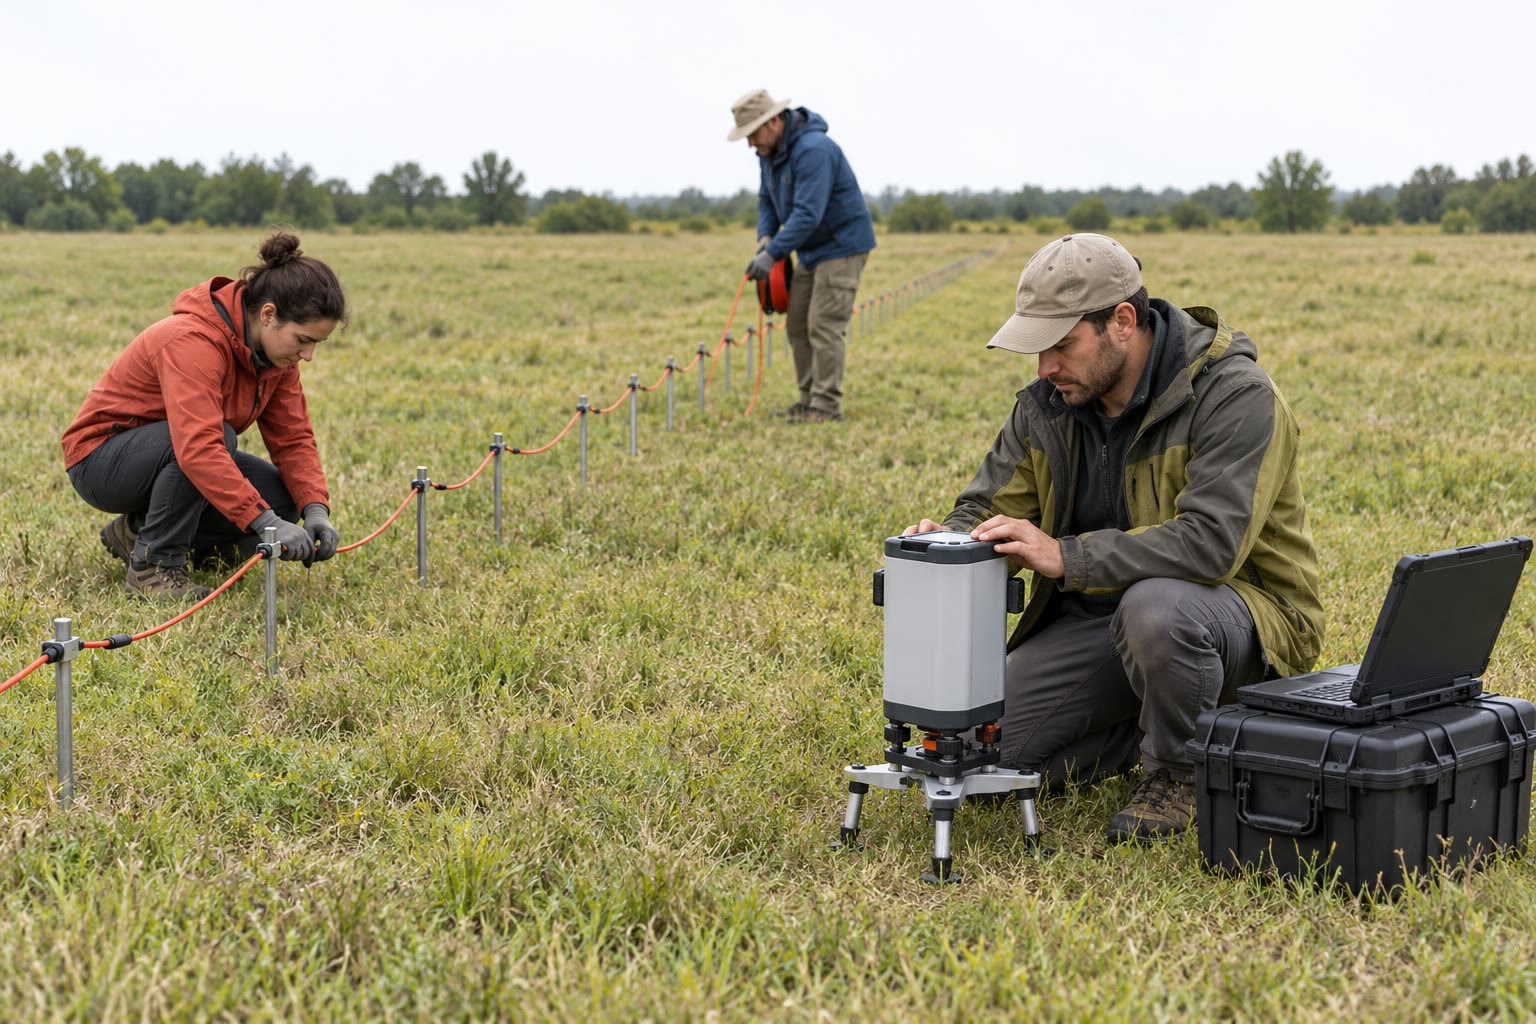
\includegraphics[width=\linewidth]{images/book5/ai/b3-geophysics-crew.jpg}

{\scriptsize एक भूभौतिकी दल प्रतिरोधकता केबल बिछा रहा है, जिसके आधार पर
एक गुरुत्वमापी रखा है (AI से बनाया गया चित्रण)।}
\end{minipage}
\end{inthefield}

\begin{example}[वार्डन सर्वेक्षण]\label{ex:b3:field-lab-methods-3:varden}
गुरुत्व मानचित्र ग्रेनाइट पर केंद्रित, लगभग \qty{-2.3}{\milli\gal} का एक बंद निम्न दिखाता है,
जो उत्तर--दक्षिण दिशा में लंबा है: हल्का ग्रेनाइट आवरण के नीचे आगे तक जाता है,
और उसी दिशा में सबसे लंबा है। यह निम्न
अनावरण से लगभग \qty{1}{km} तक फैला है, इसलिए पिंड गहराई के साथ चौड़ा होता है।
उसकी अर्ध-चौड़ाई समतुल्य गोले के लिए एक पहली गहराई देती है;
ऊर्ध्वाधर पार्श्व और तल वाले मॉडल दिखाते हैं कि एक से
कुछ किलोमीटर गहरा तल चोटी को उतनी ही अच्छी तरह समझाता है,
कुछ दसवें मिलीगल के भीतर, इसलिए तल अज्ञात रहता है---पिछले अनुभाग की अनेकमानता।
ग्रेनाइट के ऊपर घाटी के तल पर ध्वनन
सूखी बजरी की प्रतिरोधकता से शुरू होता है और वहाँ नीचे जाता है,
जहाँ धारा जल-संतृप्त जलोढ़ में प्रवेश करती है, और एक ढलान-एक की सीधी रेखा के साथ ऊपर उठता है:
एक चालक आवरण, जिसके नीचे अत्यधिक प्रतिरोधी आधार, यानी
ग्रेनाइट, कुछ मीटर नीचे है। उसी तल के साथ खींचा गया रडार
एक समतल प्रतिध्वनि लगभग \qty{20}{ns} पर दिखाता है: भौम जलस्तर। और चुंबकीय रेखा,
वलन के पश्चिमी पार्श्व के पार, जहाँ आवरण मोटा है और
आधार के शिस्ट दो सौ मीटर के आसपास नीचे पड़े हैं, एक सममित उच्च दर्ज करती है,
लगभग \qty{20}{nT} का, जिसे कोई मानचित्र नहीं समझाता: एक मैफ़िक डाइक,
मैग्नेटाइट से समृद्ध, आवरण के नीचे दबी; उसका स्ट्राइक
चुंबकीय याम्योत्तर के अनुदिश है, इसीलिए विसंगति सममित है। भूभौतिकीविद्
इसे एक डोलेराइट डाइक बताते हैं जो असंगति पर कटी है, जिसे मानचित्र का
आवरण छिपाता है। सप्ताहांत समस्या
सर्वेक्षण के आँकड़ों का संशोधन करती है।
\end{example}
% ledger: gpg:susceptibility, gpg:resistivity, gpg:gpr-table

\section{अभ्यास}

\begin{exercise}[$\star$]\label{exo:b3:field-lab-methods-3:1}
(क)~$g = \qty{9.81}{m.s^{-2}}$ का कितना भाग \qty{0.01}{\milli\gal} है?
(ख)~गुरुत्वमापी को कितना ऊपर उठाया जाए कि उसका पाठ्यांक
केवल मुक्त-वायु प्रभाव से \qty{0.01}{\milli\gal} बदल जाए? (ग)~मुक्त-वायु
और बूगेर प्रभाव दोनों एक साथ, घनत्व
\qty{2670}{kg.m^{-3}} लेकर?
\end{exercise}

\begin{exercise}[$\star$]\label{exo:b3:field-lab-methods-3:2}
त्रिज्या \qty{50}{m} और घनत्व अंतर
\qty{+500}{kg.m^{-3}} वाले एक गोले का केंद्र \qty{100}{m} गहराई पर है। उसका
अधिशेष द्रव्यमान, उसकी विसंगति की चोटी और अर्ध-चौड़ाई $x_{1/2}$ परिकलित कीजिए।
\end{exercise}

\begin{exercise}[$\star$]\label{exo:b3:field-lab-methods-3:3}
अंतराल $a = \qty{10}{m}$ वाला एक वेनर विन्यास \qty{0.1}{A} धारा प्रवाहित करता है और
\qty{0.239}{V} मापता है। (क)~ज्यामितीय गुणांक और
\omterm{def:b3:field-lab-methods-3:resistivity}{आभासी प्रतिरोधकता} परिकलित कीजिए। (ख)~दिखाइए कि $s =
\qty{15}{m}$ और $l = \qty{5}{m}$ वाले श्लमबर्गर विन्यास का ज्यामितीय गुणांक वही है, और
इसका कारण समझाइए।
\end{exercise}

\begin{exercise}[$\star$]\label{exo:b3:field-lab-methods-3:4}
ग्रेनाइट का $\varepsilon_r = 5$ है। (क)~रडार वेग परिकलित कीजिए। (ख)~एक
विभंग \qty{10}{m} नीचे है: उसकी प्रतिध्वनि का द्विमार्ग काल परिकलित कीजिए।
(ग)~$\sigma = \qty{1}{mS.m^{-1}}$ लेकर त्वचा गहराई और
लगभग तीन त्वचा गहराई जितनी उपयोगी गहराई परिकलित कीजिए। (घ)~एक गीली मिट्टी से तुलना कीजिए, जिसका
$\varepsilon_r = 20$ और $\sigma = \qty{10}{mS.m^{-1}}$ है।
\end{exercise}

\begin{exercise}[$\star\star$]\label{exo:b3:field-lab-methods-3:5}
(क)~त्रिज्या $R$ वाले एक लंबे क्षैतिज बेलन की विसंगति,
जिसका घनत्व अंतर $\Delta\rho$ है और अक्ष गहराई $z$ पर है, एक रेखीय द्रव्यमान की विसंगति से
व्युत्पन्न कीजिए और दिखाइए कि $z = x_{1/2}$। (ख)~एक बेलन और एक गोला
समान चोटी और समान अर्ध-चौड़ाई $x_{1/2} = \qty{100}{m}$ देते हैं।
उनकी गहराइयों की तुलना कीजिए। कौन-सी व्याख्या अधिक गहरा पिंड देती है?
\end{exercise}

\begin{exercise}[$\star\star$]\label{exo:b3:field-lab-methods-3:6}
वार्डन ग्रेनाइट मॉडल की बूगेर विसंगति, जिसका नमूना हर
\qty{100}{m} पर लिया गया है, \num{1120} बिंदुओं वाले एक मानचित्र पर, जो $\qty{3.5}{km}
\times \qty{3.2}{km}$ क्षेत्र को ढकता है, उनका योग \qty{-438}{\milli\gal} है। (क)~
\cref{prop:b3:field-lab-methods-3:gauss} से द्रव्यमान न्यूनता का अनुमान लगाइए।
(ख)~मॉडल की द्रव्यमान न्यूनता \qty{1.74e11}{kg} है। मानचित्र उसका कितना भाग
पुनः प्राप्त करता है, और शेष कहाँ है?
\end{exercise}

\begin{exercise}[$\star\star$]\label{exo:b3:field-lab-methods-3:7}
(क)~एक पतली डाइक का शीर्ष \qty{30}{m} नीचे है। प्रति अर्ध-चौड़ाई तीन पाठ्यांकों के नियम का उपयोग करके,
जहाँ अर्ध-चौड़ाई विसंगति की वह पूर्ण चौड़ाई है जो अपनी चोटी के आधे पर हो,
स्टेशन अंतराल कितना चाहिए? (ख)~
वही, जब शीर्ष \qty{220}{m} नीचे हो। (ग)~एक ही सर्वेक्षण उथले और गहरे पिंड दोनों को क्यों नहीं
विभेदित कर सकता, जब तक वह
उथले पिंड के लिए ही डिज़ाइन न किया गया हो?
\end{exercise}

\begin{exercise}[$\star\star$]\label{exo:b3:field-lab-methods-3:8}
\qty{8}{\ohm\metre} प्रतिरोधकता वाले पानी से संतृप्त एक बलुआ पत्थर की
प्रतिरोधकता \qty{80}{\ohm\metre} है। (क)~$a = 1$ और $m = 2$ लेकर,
उसकी छिद्रता परिकलित कीजिए। (ख)~$m = 1.8$ और $m = 2.2$ लेकर दोहराइए। कौन-सा
मापन का पद छिद्रता की अनिश्चितता को नियंत्रित करता है?
\end{exercise}

\begin{exercise}[$\star\star$]\label{exo:b3:field-lab-methods-3:9}
(क)~\cref{prop:b3:field-lab-methods-3:layers} की दो-परत श्रेणी के पहले तीन पद
$s = 2h_1$ पर $k =
\num{0.5}$ और $k = \num{-0.5}$ के लिए, तथा उनसे प्राप्त आभासी प्रतिरोधकताएँ परिकलित कीजिए।
(ख)~$\rho_a/\rho_1$ की सीमाएँ क्या हैं, जब $s \ll h_1$ और
$s \gg h_1$ हो? (ग)~कौन-से प्रतिरोधकता अनुपात $\rho_2/\rho_1$
$k = \pm 0.5$ के अनुरूप हैं?
\end{exercise}

\begin{exercise}[$\star\star\star$]\label{exo:b3:field-lab-methods-3:10}
(क)~वेन्नर विन्यास का ज्यामितीय गुणक
\cref{thm:b3:field-lab-methods-3:point-source} से व्युत्पन्न कीजिए। (ख)~श्लमबर्जर विन्यास का गुणक भी व्युत्पन्न कीजिए, और
दिखाइए कि $\rho_a \to 2\pi s^2(-\mathrm{d}V/
\mathrm{d}r)/I$ जब $l/s \to 0$। (ग)~सन्निकट
गुणक $\pi s^2/(2l)$ सटीक मान को, जब $l = s/10$ हो, कितना अधिक आँकता है?
\end{exercise}

\begin{exercise}[$\star\star\star$]\label{exo:b3:field-lab-methods-3:11}
एक स्टेशन आधार से \qty{50}{m} ऊपर स्थित है। इसका पाठ्यांक
\qty{0.01}{\milli\gal} तक सही है, इसकी ऊँचाई \qty{5}{cm} तक; स्लैब का घनत्व
\qty{100}{kg.m^{-3}} तक अनिश्चित है और \omterm{def:b3:field-lab-methods-3:terrain}{भू-भाग संशोधन}
\qty{0.2}{\milli\gal} तक। (क)~इसकी बूगेर विसंगति का त्रुटि-बजट तैयार कीजिए।
(ख)~कौन-सा पद प्रबल है, और \qty{0.1}{\milli\gal} की विसंगति पहचानने
के लिए किस पद में सुधार करेंगे? (ग)~भू-भाग पद के बिना
कुल मान क्या है?
\end{exercise}

\begin{exercise}[$\star\star\star$]\label{exo:b3:field-lab-methods-3:12}
दबे हुए पिंड के आर-पार पाँच गुरुत्व पाठ्यांक, $x = -600$, $-300$, $0$,
$300$ और \qty{600}{m} पर, \num{-0.69}, \num{-2.17}, \num{-4.16},
\num{-2.10} और \qty{-0.73}{\milli\gal} हैं, प्रत्येक का $\sigma =
\qty{0.03}{\milli\gal}$ है। (क)~$x = 0$ के नीचे केंद्रित गोलक मॉडलों के लिए
\num{300}, \num{400} और \qty{500}{m} गहराई पर, वह द्रव्यमान चुनिए जो
केंद्रीय पाठ्यांक से मेल खाए, और प्रत्येक का \omterm{def:b3:field-lab-methods-3:inversion-practice}{बेमेल} $\chi^2$ परिकलित कीजिए। (ख)~कौन-सा
मॉडल आँकड़ों से उनकी त्रुटियों के भीतर मेल खाता है? (ग)~क्या अन्य आकार का
पिंड भी उतना ही मेल खा सकता है? किस बात से निर्णय होगा?
\end{exercise}

\section{समस्या: वार्डन पहाड़ियों के छिपे हुए पिंड}

\begin{problem}[{सप्ताहांत समस्या --- वार्डन सर्वेक्षण का समानयन}]
\label{pb:b3:field-lab-methods-3:1}
$G = \qty{6.674e-11}{m^3.kg^{-1}.s^{-2}}$, मुक्त-वायु प्रवणता
\qty{0.3086}{\milli\gal.m^{-1}} और बूगेर गुणांक
\qty{0.1119}{\milli\gal.m^{-1}} (घनत्व \qty{2670}{kg.m^{-3}}) का प्रयोग कीजिए।

\medskip\noindent\textbf{भाग I --- एक गुरुत्व लूप।} गुरुत्व प्रोफ़ाइल पर एक लूप
के माप (अंशांकन के बाद मिलीगैल में पाठ्यांक, मीटर में ऊँचाइयाँ,
और 09:00 के बाद घंटों में समय) देता है:
\begin{center}
\small
\begin{tabular}{lccccc}
\hline
स्टेशन & आधार & \qty{3.0}{km} & \qty{3.5}{km} & \qty{4.0}{km} & आधार \\
\hline
समय & 0 & 0.5 & 0.9 & 1.3 & 2.0 \\
ऊँचाई & 176.1 & 149.0 & 145.5 & 158.0 & 176.1 \\
पाठ्यांक & 2846.512 & 2851.075 & 2850.497 & 2849.392 & 2846.708 \\
\hline
\end{tabular}
\end{center}
\begin{enumerate}
\item लूप की विचलन दर परिकलित कीजिए।
\item विचलन के लिए तीनों स्टेशन पाठ्यांकों का संशोधन कीजिए और उन्हें
  आधार के सापेक्ष व्यक्त कीजिए।
\item ऊँचाई के अंतरों के लिए मुक्त-वायु सुधार और बूगेर सुधार लागू कीजिए,
  और प्रत्येक स्टेशन की
  आधार के सापेक्ष बूगेर विसंगति दीजिए।
\item केवल उपकरण का विचलन \qty{0.040}{\milli\gal.h^{-1}} था।
  आधार पर हुए परिवर्तन का शेष भाग किस कारण से हुआ, और वह
  विचलन के साथ ही क्यों हटाया जा सकता था?
\item जिस मॉडल से ये पाठ्यांक आए हैं, वह तीनों विसंगतियाँ
  आधार के सापेक्ष \num{-0.825}, \num{-2.131} और
  \qty{-0.825}{\milli\gal} देता है। समानयन की त्रुटियाँ परिकलित कीजिए। तालिका की
  ऊँचाइयाँ \qty{0.1}{m} तक पूर्णांकित हैं: इस पूर्णांकन से कौन-सी त्रुटि आ सकती है,
  और क्या यह त्रुटियों की व्याख्या करता है?
\item कितनी ऊँचाई-शुद्धता समानीत विसंगति को
  \qty{0.01}{\milli\gal} के भीतर रखती है? सर्वेक्षण नियमावलियाँ
  \qty{3.3}{cm} क्यों माँगती हैं, जो एक अधिक कड़ा मान है?
\end{enumerate}

\medskip\noindent\textbf{भाग II --- ग्रेनाइट की विसंगति।} प्रोफ़ाइल के साथ विसंगति का
न्यूनतम \qty{-2.293}{\milli\gal} है, और यह
$x = \qty{3.50}{km}$ पर है, तथा उसका आधा मान $x = 3.048$ और
\qty{3.952}{km} पर पार करती है। ग्रेनाइट मॉडल का घनत्व-अंतर
\qty{-130}{kg.m^{-3}} है, और केंद्र पर भूमि \qty{145.5}{m}
समुद्र-तल से ऊपर है।
\begin{enumerate}[resume]
\item अर्ध-चौड़ाई $x_{1/2}$ और तुल्य गोले के केंद्र की
  गहराई परिकलित कीजिए।
\item उस गोले की द्रव्यमान-न्यूनता, और ग्रेनाइट के घनत्व-अंतर के लिए उसकी
  त्रिज्या परिकलित कीजिए। परिणाम में क्या अजीब है?
\item मॉडल का द्रव्यमान-केंद्र भूमि से \qty{864}{m} नीचे है, और उसकी
  द्रव्यमान-न्यूनता \qty{1.74e11}{kg} है। अर्ध-चौड़ाई नियम क्यों
  एक अधिक उथला और हल्का पिंड देता है?
\item असंगति पर ग्रेनाइट के समान क्षेत्रफल वाला एक ऊर्ध्वाधर बेलन
  की त्रिज्या \qty{461}{m} है। इसकी अक्ष पर विसंगति, जब ऊपरी सिरा
  भूमि पर हो और तल \qty{1645}{m} गहराई पर हो, तथा असीमित गहराई के लिए
  परिकलित कीजिए।
\item परीक्षण या हल करके वह तल-गहराई ज्ञात कीजिए, जिस पर यह
  बेलन प्रेक्षित विसंगति \qty{-2.29}{\milli\gal} देता है।
\item जब उसका ऊपरी सिरा \qty{6}{m} नीचे हो, तब बेलन की विसंगति
  परिकलित कीजिए (तल \qty{1645}{m})। क्या गुरुत्व यह बता सकता है कि ग्रेनाइट
  जलोढ़ के नीचे सतह तक पहुँचता है या नहीं?
\end{enumerate}

\medskip\noindent\textbf{भाग III --- घाटी का तल।} ग्रेनाइट के ऊपर के तल पर
श्लमबर्जर ध्वनन (अर्ध-अंतराल $s$ मीटर में,
$\rho_a$ \unit{\ohm\metre} में) देता है:
\begin{center}
\small
\begin{tabular}{lcccccccc}
\hline
$s$ & 1 & 2 & 4 & 6 & 10 & 20 & 30 & 40 \\
$\rho_a$ & 577 & 526 & 387 & 350 & 449 & 821 & 1309 & 1684 \\
\hline
\end{tabular}
\end{center}
उसी तल के साथ एक रडार प्रोफ़ाइल पर एक पाइप एक हाइपरबोला देता है, जिसका
शीर्ष \qty{10.7}{ns} पर है, और \qty{1}{m} दूर पर समय \qty{17.1}{ns} है;
एक समतल प्रतिध्वनि \qty{20.0}{ns} पर पहुँचती है।
\begin{enumerate}[resume]
\item $s = \qty{20}{m}$ पर MN की लंबाई \qty{2}{m} थी, और धारा
  \qty{50}{mA} थी। ज्यामितीय गुणक और मापी गई वोल्टता परिकलित कीजिए।
\item रडार वेग, जलोढ़ की सापेक्ष विद्युतशीलता
  और पाइप की गहराई परिकलित कीजिए।
\item समतल प्रतिध्वनि भौम जलस्तर है। यह कितनी गहरी है?
\item 20, 30 और
  \qty{40}{m} पर पाठ्यांकों से जलोढ़ की चालकता $S$ का अनुमान लगाइए।
\item शुष्क जलोढ़ की प्रतिरोधकता \qty{600}{\ohm\metre} है, और संतृप्त
  जलोढ़ \qty{222}{\ohm\metre} है। संतृप्त जलोढ़ की मोटाई
  और ग्रेनाइट के शीर्ष की गहराई परिकलित कीजिए। यह अनुमान उच्च है या निम्न,
  और क्यों?
\item भूजल की प्रतिरोधकता \qty{20}{\ohm\metre} है। \omterm{prop:b3:field-lab-methods-3:archie}{आर्ची नियम} से
  $m = 2$ लेकर जलोढ़ की छिद्रता, और $m$ का परास
  \num{1.3} और \num{2.8} के बीच परिकलित कीजिए।
\end{enumerate}

\medskip\noindent\textbf{भाग IV --- चुंबकीय रेखा।} रेखा
पूर्व की ओर $x = \qty{1.70}{km}$ से चलती है, हर \qty{50}{m} पर एक स्टेशन और हर
दो मिनट पर; आधार स्टेशन उन्हीं मिनटों पर दर्ज करता है। पाठ्यांक,
\qty{48000}{nT} घटाने के बाद, ये हैं:
\begin{center}
\small
\setlength{\tabcolsep}{3.5pt}
\begin{tabular}{lccccccccccc}
\hline
$x$ (km) & 1.70 & 1.75 & 1.80 & 1.85 & 1.90 & 1.95 & 2.00 & 2.05 & 2.10 & 2.15 & 2.20 \\
रेखा & 3.4 & 4.8 & 6.3 & 8.1 & 10.3 & 12.8 & 15.8 & 19.2 & 22.9 & 26.2 & 28.0 \\
आधार & 0.0 & 0.7 & 1.5 & 2.2 & 2.9 & 3.6 & 4.3 & 5.0 & 5.7 & 6.4 & 7.0 \\
\hline
$x$ (km) & 2.25 & 2.30 & 2.35 & 2.40 & 2.45 & 2.50 & 2.55 & 2.60 & 2.65 & 2.70 & \\
रेखा & 27.7 & 25.8 & 23.3 & 20.9 & 19.0 & 17.6 & 16.6 & 15.9 & 15.5 & 15.2 & \\
आधार & 7.6 & 8.2 & 8.8 & 9.4 & 9.9 & 10.4 & 10.9 & 11.3 & 11.7 & 12.1 & \\
\hline
\end{tabular}
\end{center}
मुख्य क्षेत्र \qty{48000}{nT} है, जो \ang{65} पर झुका हुआ है।
\begin{enumerate}[resume]
\item \omterm{def:b3:field-lab-methods-3:magnetic}{दैनिक संशोधन} लागू कीजिए और प्रत्येक स्टेशन पर
  संशोधित विसंगति ज्ञात कीजिए।
\item दिखाइए कि संशोधन के बिना विसंगति कभी
  पूर्वी पक्ष पर अपने शिखर के आधे तक नहीं गिरती।
\item शिखर और वे दो बिंदु ज्ञात कीजिए जहाँ संशोधित विसंगति
  शिखर की आधी है, रैखिक अंतर्वेशन द्वारा, और अर्ध-चौड़ाई परिकलित कीजिए।
\item विसंगति सममित है। इससे पिंड के स्ट्राइक के बारे में
  क्या निष्कर्ष निकलता है, और अर्ध-चौड़ाई नियम किस प्रकार के पिंड को मानता है?
\item चुंबकीय प्रवृत्ति और मोटाई का गुणनफल $\kappa t$ परिकलित कीजिए।
  यदि डाइक \num{0.03} चुंबकीय प्रवृत्ति वाला डोलेराइट है, तो वह
  कितनी मोटी है?
\item क्या स्टेशन पर्याप्त पास-पास थे?
\item भूमि के नीचे छिपे डाइक के शीर्ष की गहराई
  निकटतम दस मीटर तक दीजिए, और उसकी तुलना क्षेत्र के भूवैज्ञानिक मॉडल
  पर असंगति की गहराई से कीजिए, जो इस
  बिंदु पर \qty{222}{m} है।
\end{enumerate}
\end{problem}
% ledger: gpg:grav-survey, gpg:mag-field, keys:archie
